\chapter{Feature Design} \label{sec:feature}
	% Chapter overview of sections

	% Introduction into sections
	\section{System Overview}

		\paragraph{What is OASIS}

		\paragraph{Objective}

		\paragraph{Virtual Heliodon Pipeline}

			Both OASIS and the Virtual Heliodon provide a solution the problem of daylighting analysis during the early stage of architectural design.
			In addition to sharing the same objectives both OASIS and the Virtual Heliodon utilize the physical sketch interpretation algorithm and the daylight rendering engine.
			As a result it can be difficult to see where these two systems vary.
			In order to understand the contributions I made to OASIS we must briefly cover the system pipeline of the Virtual Heliodon.
			The Virtual Heliodon's system pipeline is illustrated in Figure-\ref{pipeline_vh}.
			To begin, the Virtual Heliodon features a novel tangible user interface for the creation of architectural spaces.
			Users define architectural spaces by manipulating physical foam primitives with their hands.
			After users are satisfied with their architectural space they can either use a wireless clicker or communicate to the operator to run the \textit{table top detect processes} and continue down the pipeline.
			The \textit{table top detect} processes is a simple computer vision program that takes an overhead image of the foam primitives and detects where those primitive are in an image.
			The coordinates of where those primitives are in an image are stored in an intermediary primitives file. The intermediary primitives file is used as input for the physical sketch interpretation algorithm. As mentioned previously, the physical sketch interpretation algorithm generates a closed watertight triangle mesh.
			Currently, there exist no user interface for the generation of daylight renderings.
			Instead an operator familiar with the system is required to generate visualizations for the users. A user would communicate to the operator and the operator would alter scripts in order to generate rendered image textures and project onto the foam primitives. Both places in the system time pipeline that require an operator is illustrated in Figure-\ref{pipeline_vh}A-B.

			Accordingly, OASIS varies from the Virtual Heliodon in three main aspects.

			Firstly, OASIS uses a sketching interface rather than tangible user interface;
			the sketching interface does not limit users to the number of foam primitives available, nor does the sketching interface limit users to discrete wall and window lengths.
			Additionally, because our sketching interface is in software we can directly convert user sketches into intermediary primitive files. However, the Virtual Heliodon requires stable lighting conditions for top top detect processes to locate primitives in an overhead photograph of a users design.
			Interestingly, OASIS also does not have to worry failure to locate primitives due to occlusions in the overhead image taken of users models.
			Secondly, our solution is entirely software. OASIS does not feature an feature an augmented reality system.
			As a result OASIS does not have to tackle the problem of projector coverage \cite{sheng2009virtual} or diffcculites of color bleeding of super imposed textures on foam primatives\cite{sheng2011perceptual}.
			Lastly, OASIS is fully autonomous and does not require an operator or programing experience to use.









  		\begin{figure}[h]
			\centering
			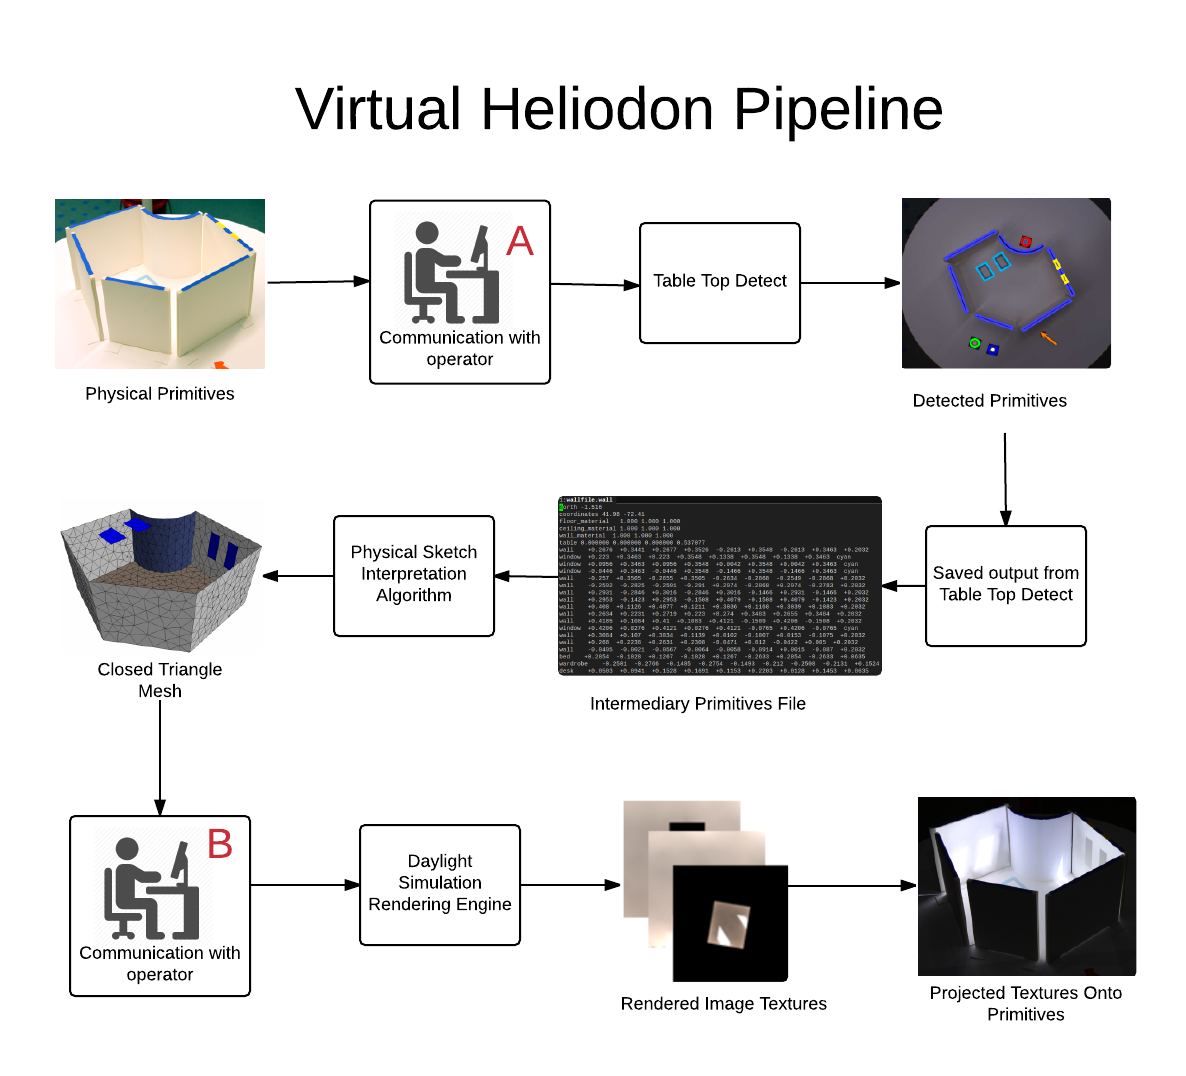
\includegraphics[width=1.0\textwidth]{pipeline_vh}
			\caption{Virtual Heliodon's Simplified Pipeline.}
			\label{fig:new_pipeline}
			\end{figure}








		\paragraph{OASIS Pipeline}

			OASIS is an alternative interface to the Virtual Heliodon. 
			The system pipeline in Figure-\ref{fig:new_pipeline} illustrates the components involved in OASIS.
			In addition, Figure-\ref{fig:new_pipeline} emphasizes all portions of OASIS that I directly contributed to.
			% Grammar checkpoint
			The physical sketch interpretation algorithm that the Virtual Heliodon uses to generate watertight 3D meshes for simulations require sketches be given as a collection of model primitives. 
			Model primitives are stored in an intermediary primitives file where each line describes a wall,window, or furniture item in a sketch.
			In the Virtual Heliodon the intermediary primitives file is created by a simple computer vision algorithm that detects walls, windows, and tokens through colored markers placed on the top of all physical primitives.
			In our sketching interface I directly create this intermediary primitives file through the conversion of user created Raphael Objects.
			Figure-\ref{fig:new_pipeline}A illustrates where the conversion occurs in our system pipeline.
			When users convert their sketches into 3D models, the physical sketch interpretation algorithm reads in the generated intermediary primitives file.
			The physical sketch interpretation algorithm outputs a closed triangle mesh that the user can view in the \textit{Generate 3D Model} page.
			Given confirmation that a 3D generated model matches user's intention, the user can create a daylight simulation request in the \textit{Create Daylighting Simulation} page.
			This portion of the system pipeline is illustrated in Figure-\ref{fig:new_pipeline}B.
			After the submission of a daylight simulation request, I use the daylight simulation rendering engine to produce texture images.
			These texture images capture illumination in a viewpoint independent manner.
			On the \textit{Analyze Daylighting} page, I map these texture images onto the 3D mesh to display a daylight rendering of the user's generated model.
			Figure-\ref{fig:new_pipeline}C illustrates where texture mapping occurs in the system pipeline.
			In brief, our pipeline shows that OASIS is an alternative interface to the physical sketch interpretation algorithm and daylight rendering engine in the Virtual Heliodon.

			\begin{figure}[h]
			\centering
			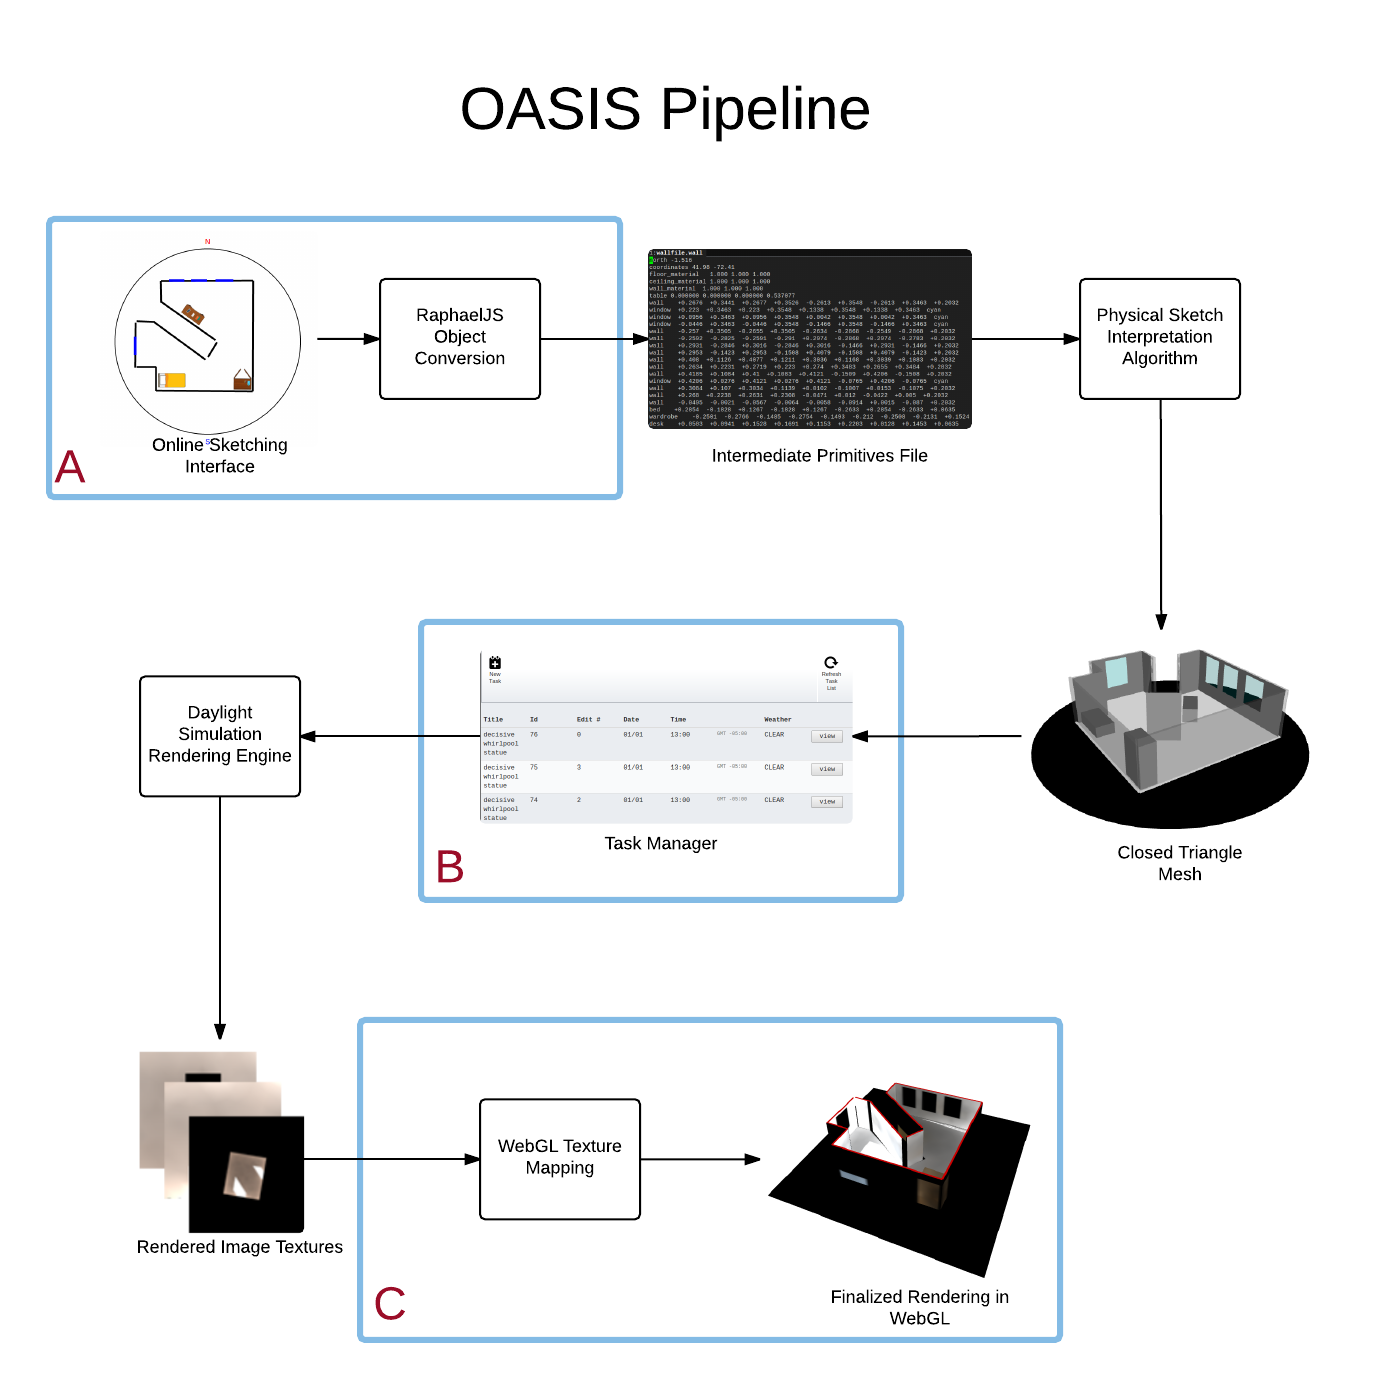
\includegraphics[width=1.0\textwidth]{new_pipeline}
			\caption{OASIS pipeline diagram with the author's contributions noted in blue.}
			\label{fig:new_pipeline}
			\end{figure}

		\paragraph{Importance of good UI}

	\section{Sketching Interface Design}
		\paragraph{Sketching Walls and Windows}
			% Why is sketching walls/win important
			% Discussion about what we do
			% Discussion about alternatives(old method)
			% Discussion about Eric's work
		\paragraph{Furniture Placement}
			% Why is furniture important
				% Scale
				% Meaning (identity)
				% Relate to space
			% Discussion about how we place furniture
			% Discussion about furture work on sketched furniture items
				% Dynamic scale??
		\paragraph{Removal of Elements}
			% Why is removal important
				% side: machines do better removal than pen & paper
			% How do we implement it
			% Alternatives
		\paragraph{Cardinal Orientation}
			% Why is orientation important
			% How do we implement it? 
			% Alternatives
		\paragraph{Geographical Positioning}
			% Why is location important
			% How do we implement it? 
			% Alternatives

	\section{3D model viewer}

		\subsection{Physical Sketch Interpretation Algorithm Viewer}
			\paragraph{Intention}
			\paragraph{Examples of successful interpretations}
			\paragraph{Examples of unsuccessful interpretations}

		\subsection{Daylight Rendering engine viewer}
			\paragraph{Examples of successful interpretations}
			\paragraph{Examples of unsuccessful interpretations}
				\paragraph{Examples of over illuminatioh}
				\paragraph{Examples of under illuminatioh}

		\subsection{Share a Model viewer}
			\paragraph{Purpose of Model Viewer}
			\paragraph{Alternatives?}

	\section{Web Application Design}
		\paragraph{Why is good UI important for our application}
		\paragraph{General User Interface choices}
		\paragraph{Non-Linearity in OASIS}
		\paragraph{Loading Previous Models and Rendering Task}

	\section{Problems Encountered}
		\paragraph{Computational Intensive Procedures}
		\paragraph{Saving Models Safety}
		\paragraph{Dealing with Clueless Users}

	\section{Implementation}

		\subsection{Frameworks Used}
			\paragraph{WebGL}
			\paragraph{RaphaelJS}
				Another framework used in our sketching interface is RaphaelJS\cite{todo}.
				Raphael JS is a 3D vector graphics library for JavaScript. 
				I use RaphaelJS to create 2D graphics of objects users places into sketches. I also use RaphaelJS because it supports vectorized lines and shapes, allowing our interface  to be re-sizable with lost of visual quality.
				I also use Raphael FreeTransform in conjunction with RaphaelJS\cite{todo}. 
				The FreeTransform extension is used to create FreeTransform handles on furniture items so that users may easily rotate and reposition furniture items where they please.
				Figure-\ref{fig:oldvh}F demonstrates the handles FreeTransform generates for object manipulation.\\


			\paragraph{RibbonJS}


		\subsection{Window Snapping}

	\section{Chapter Summary}
		% Summary of what we covered

